\section{Differential cross-section}

%----------------------------------------------------------------------------------------------------
\subsection{Event reconstruction}

One arm
\begin{equation}
\label{eq:kin 1a}
	\begin{aligned}
		\theta_x^* &= {v_x^{\rm N} x^{\rm F} - v_x^{\rm F} x^{\rm N}\over v_x^{\rm N} L_x^{\rm F} - v_x^{\rm F} L_x^{\rm N}}\ ,\qquad
		\theta_y^* = {1\over 2} \left( {y^{\rm N}\over L_y^{\rm N}} + {y^{\rm F}\over L_y^{\rm F}} \right)\ ,\\
		x^* &= {L_x^{\rm N} x^{\rm F} - L_x^{\rm F} x^{\rm N}\over L_x^{\rm N} v_x^{\rm F} - L_x^{\rm F} v_x^{\rm N}}\ , \\
	\end{aligned}
\end{equation}

two arm
\begin{equation}
\label{eq:kin 2a}
	\begin{aligned}
		\theta_x^* &= {
				\sum v_i^2 \sum L_i x_i - \sum L_i v_i \sum v_i x_i
				\over
				\sum v_i^2 \sum L_i^2 - \sum L_i v_i \sum L_i v_i
			}\ ,\\
		\theta_y^* &= (\theta_y^{*L} + \theta_y^{*R})/2\ .\\
	\end{aligned}
\end{equation}

%------------------------------
{\bf Alignment}

\> the three methods: collimation, track-based and with physics processes

\> the new approach for alignment with elastics
\>> excellent for relative alignment (between near and far or left and right)
\>> absolute (= wrt.~the beam) achieved with the right arm and two complementary methods:

\noindent 1) standard method with vertical RPs
\noindent 2) fitting the axis of diffractive-proton axis and extrapolation to beam position

\> final uncertainty, also propagated to $\theta^*_{x, y}$ angles

\> the observed hit inefficiencies -- possible asymmetries -- discuss ???
\> mention final alignment check = 2D Gaussian fit of $\theta_x^*$ vs.~$\theta_y^*$ from both diagonals ??

%------------------------------
{\bf Optics}

\> choice of reconstruction formulae in x and in y
\>> guide = robustness against error sources: beam divergence, sensor pitch, misalignment, vertex term neglected, optics imperfections
\>> two types of reconstruction: one-arm (for cuts) and two-arm (for physics)
\>> TODO: what reco formulae used

\> typical values of uncertainties: statistical (smearing) and systematic (optics, ...)


%------------------------------
{\bf Resolution}


%----------------------------------------------------------------------------------------------------
\subsection{Differential cross-section}

{\bf Tagging}. The cuts used to select the elastic events are summarized in Tab.~\ref{tab:cuts}, all are applied at $4\sigma$-level. Cuts 1 and 2 require the reconstructed-track collinearity between the left and right arm. Cut 3 ensures that the protons come from the same vertex (horizontally). \todo{why only three cuts}: sufficient -- collinearity very powerful!
\todo{TODO: update} The tagging efficiency is studied by applying the cuts also at $5\un{\sigma}$-level. This selection yields $0.5\un{\%}$ more events, uniformly in $|t|$ -- thus the inefficiency is irrelevant for this analysis.

\begin{table}
\caption{The elastic selection cuts. The superscripts R and L refer to the right and left arm. The right-most column gives a typical RMS of the cut distribution.
}
\label{tab:cuts}
\begin{center}
\vskip-3mm
\begin{tabular}{ccc}\hline\hline
number & cut & RMS ($\equiv 1\sigma$)\cr\hline
1 & $\theta_x^{*\rm R} - \theta_x^{*\rm L}$				& $3.9\un{\mu rad}$	\cr
2 & $\theta_y^{*\rm R} - \theta_y^{*\rm L}$				& $1.0\un{\mu rad}$	\cr
3 & $x^{*\rm R} - x^{*\rm L}$							& $TODO\un{\mu m}$ 	\cr\hline\hline
\end{tabular}
\end{center}
\end{table}

\> the three main cuts: left-right collinearity in $x$ and $y$, left-right vertex $x^*$ comparison
\>> motivation, sigmas
\> applied at 4 sigmas ??
\> inefficiency of the cuts (how many true events lost)

\> control cuts (not applied, used for validation only): $y^{N}$ vs.~local $\theta_y$ correlation, reconstructed $x^*$ compatible with vertex distribution?


%-------------------------
{\bf Background}

\> background = impurity of the cuts above

\> method: plot a cut quantity under various cuts
\>> central peak (signal) stays
\>> tails (background) drop
\>> residual after all cuts $\rightarrow$ interpolate to signal region $\rightarrow$ background negligible
\>> can be repeated for any cut -- compatible results ??

\> further test: $|t|$-distributions under various combinations of cuts -- background distributed uniformly over $|t|$, no peaking

%-------------------------
{\bf Acceptance correction}

\> ``standard procedure'' (ref. to previous publications?): ``divergence'' and ``phi'' corrections

\> also applied $-50 < \theta_x^* < 80\un{\mu rad}$ selection to avoid the regions affected by the horizontal RPs


%-------------------------
{\bf Efficiency corrections}

\> ``standard procedure'' for the standard contributions (ref. to previous publications?): ``3-out-of-4'' (uncorrelated 1-RP inefficiencies), ``shower in near'' (near-far correlated) and ``pile-up'' (coincidence with beam-halo or any other particle)

\> 3-out-of-4 results
\>> right arm: typical results (near $\approx 98\un{\%}$, far $\approx 96.5\un{\%}$ efficiency)
\>> left arm: efficiency in far RP unexpectedly low ($\approx 90\un{\%}$) -- due to showers in horizontal RPs (horizontal in left arm closer that in the right one) -- but experimentally determinable and thus fully correctable

\> pile-up results shown in Fig.~\ref{fig:overview}
\>> strong time-dependece: linear rise within the data-taking periods, decrease in beam cleanings


%-------------------------
{\bf Unsmearing}

\> ``standard procedure'' (ref. to previous publications?)

\> but time-dependent smearing sigma, determined from the variation of $\theta_y^{*R} - \theta_y^{*L}$
\>> mention the subtlety with $\sigma(\theta_x^*)$ ?? Cannot be measured directly. The only handle comes from the emittances (crude only). But (at least for low-$|t|$), the impact of $\theta_x^*$ smearing is small -- the value of $\theta^*$ is mostly made by $\theta_y^*$, therefore $\theta_x^*$ must be very small. Consequently, $\Delta t_x = 2 \theta_x^* \Delta \theta_x^* \approx 0$

\> due to the very small beam divergence, the effect is negligible for all bins except the low-$|t|$ ones where the rapid cross-section growth appears because of the Coulomb interaction

%-------------------------
{\bf Normalisation}. Same integral between $|t| = 0.014$ and $0.2030\un{GeV^2}$ as DS1 from \cite{prl111}, where luminosity-independent calibration was applied. Leading uncertainty: $4.2\un{\%}$ from luminosity-independent method. \todo{transfer negligible?}


%-------------------------
{\bf Binning}

\> ob-3-4

%-------------------------
{\bf Systematic uncertainties}

\> ``standard procedure'' (ref. to previous publications?) of uncertainty assessment

\> leading uncertainties: residual misalignment (very low-$|t|$), normalisation (flat)

\> compatible results obtained if data right after or right before beam cleaning are used



%----------------------------------------------------------------------------------------------------
\subsection{Final data merging}

\> merging datasets + diagonals

\> central values

\> statistical uncertainties

\> systematic uncertainties


\begin{table*}
\vskip-5mm
\caption{%
\todo{TODO}: The elastic differential cross-section as determined in this analysis using the optimised binning. The left-most three columns describe bins in $t$. The representative point give the $t$ value suitable for fitting
\cite{lafferty94}. %uncertainty due to different fit models negligible:$10^{-7}\un{GeV^2}$
TODO: optimise number of digits, spacing.
}
\vskip-3mm
\label{tab:data}
\begin{center}
\input data_table.tex
\end{center}
\vskip-10mm
\end{table*}


\begin{figure*}
\begin{center}
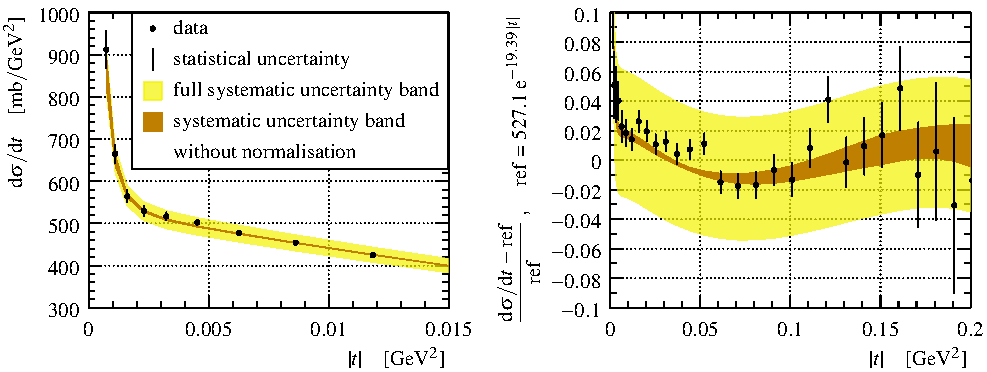
\includegraphics[width=18cm]{fig/t_dist_tabulation.pdf}
\vskip-3mm
\caption{Differential cross-section. \todo{shall we keep all 3?} \todo{describe!}}
\label{fig:dsdt}
\end{center}
\end{figure*}

\> present/comment Fig.~\ref{fig:dsdt}


